\section{Data warehouse}

\begin{definition}[\textit{Online Transaction Processing}]
    Online Transaction Processing refers to the systems that handle day-to-day transactions at operational sites.
\end{definition}
\begin{definition}[\textit{Online Analytical Processing}]
    Online Transaction Processing refers to systems designed to process and analyze data stored in large, integrated data warehouses.
\end{definition}
\noindent In general, IT systems can be categorized into two types: transactional and analytical. 
Online Transaction Processing systems typically serve as the source of data for data warehouses, while Online Transaction Processing systems are used to analyze that data.

The challenge in modern data analytics lies in integrating diverse data sources, ensuring the extraction of coherent insights, and handling the heterogeneity and distribution of data. 
Traditionally, analytics approaches have been divided into two main categories: transactional and analytical. 
The traditional query-driven approach to analytics tends to be reactive, often lazy, and on-demand, meaning data is accessed only when needed and queries are executed as they arise.

In contrast, the warehousing approach integrates data in advance, storing it in a data warehouse where it can be directly queried and analyzed. 
It offers high query performance, though it may not always provide the most up-to-date information. 
Since the data warehouse operates separately from operational systems, it doesn't interfere with local processing. Complex queries are executed within the warehouse, while operational systems continue their tasks without disruption. 
Additionally, the data stored in the warehouse can be modified, annotated, summarized, and restructured as needed, and historical information can be preserved for analysis.
However, the query-driven approach still proves more suitable in certain scenarios. 
\begin{definition}[\textit{Data warehouse}]
    A data warehouse is a collection of data that is subject-oriented, integrated, time-varying, and non-volatile, primarily used to aid decision-making within an organization.    
\end{definition}
The data warehouse is not just a simple repository; it integrates diverse datasets from various sources into a single storage location, allowing for advanced analysis and decision support.
Unlike transactional databases, data warehouses are optimized for analytical queries, not day-to-day transactions. 
They often include a user interface tailored to executives, managers, and analysts, enabling efficient decision-making.

One key characteristic of data warehouses is their ability to handle large volumes of data, often measured in gigabytes or terabytes. 
These systems are non-volatile, meaning they store historical data that doesn't change frequently. 
Updates are typically infrequent, with some warehouses being append-only, meaning that new data is added rather than modifying existing data.

\paragraph*{Architecture}
In a single-layer architecture, each data element is stored only once, with no redundancy. 
A virtual warehouse, on the other hand, presents views over operational databases without physically storing the data. 
In more common two-layer architectures, real-time data is combined with derived data for analysis. 
A three-layer architecture includes conceptual views, separating them from the transformation processes that prepare the data for querying.

\paragraph*{Decision Support Systems}
Data warehousing plays a crucial role in Decision Support Systems, which help knowledge workers. 
Online Analytical Processing is a vital component of Decision Support Systems, providing the tools to interact with and analyze data stored in the warehouse.

Relational database management systems are often used as servers for data warehouses, though flat files are less common. 
Online Transaction Processing systems come in two forms: Relational Online Transaction Processing and Multidimensional Online Transaction Processing. 
ROnline Transaction Processing uses relational databases to store and manage data warehouse content, with specialized middleware to support Online Transaction Processing functionality. 
Multidimensional Online Transaction Processing, on the other hand, uses array-based storage and offers direct access to multidimensional data, making it highly efficient for complex analytical queries.

\paragraph*{Data mart}
When comparing a data warehouse with data marts, the key difference lies in scope.
An enterprise data warehouse is an organization-wide solution that consolidates information across all departments.
In contrast, data marts focus on specific departmental needs, such as marketing or sales.
While data marts can be rolled out quickly and efficiently, they can create challenges in integration over time, particularly as multiple marts need to be synchronized.

\paragraph*{Virtual warehouse}
A virtual warehouse allows views to be created over operational databases, making it easy to query and analyze data without physically storing it in a central repository. 
However, materializing selected summary views to optimize query processing can place considerable demands on the operational databases.

\subsection{Model}
In a data warehouse, the typical structure used to organize the data is the star schema, which differs significantly from the class entity relationship diagram often used in transactional systems. 
The star schema is designed to optimize querying and analysis, providing a straightforward and efficient way to access large volumes of data.

In addition to the star schema, the snowflake schema is another common structure, which involves normalizing the dimensions of the data to reduce redundancy. 
This schema is often used when there are hierarchical relationships in the data, such as categories or time periods, that benefit from a more organized, normalized approach.

When dealing with hierarchical data, certain operations become essential for effective analysis. 
One such operation is drill-down, which involves adding one more analysis dimension, typically to disaggregate the data and view it in finer detail. 

On the other hand, roll-up is the inverse operation, where one analysis dimension is removed to aggregate the data at a higher level. 
This might involve summarizing daily sales data into weekly or monthly totals, providing a broader perspective on trends.

Another important concept in data warehousing is the datacube, which enables users to slice and dice the data, examining it from different angles by selecting specific dimensions. 
The datacube allows for complex multidimensional analysis, making it easier to explore the data and uncover insights by focusing on different combinations of dimensions.

\subsection{Snowflake}
Snowflake is an enterprise-ready cloud data warehouse solution that is designed to automatically scale in order to balance performance and costs efficiently. 
One of its major advantages is the separation between compute and storage. Unlike other databases that combine the two, Snowflake allows for independent scaling of compute and storage resources. 
This means you don't need to size your entire system for your largest workload, which helps avoid unnecessary costs.
Additionally, Snowflake provides a single place for storing all types of data, making it easier to manage and analyze large volumes of information.
\begin{figure}[H]
    \centering
    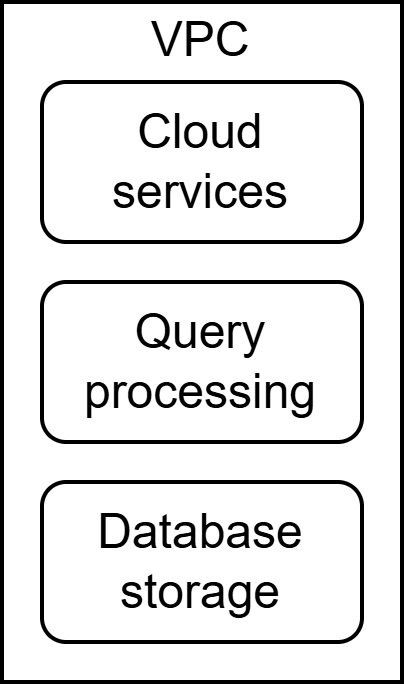
\includegraphics[width=0.25\linewidth]{images/arc.png}
    \caption{Snowflake architecture}
\end{figure}
The architecture of Snowflake is designed to optimize performance, scalability, and flexibility. It consists of three main layers:

\begin{enumerate}
    \item \textit{Database storage}: Snowflake organizes data in an internal, optimized, compressed, columnar format. 
        The system handles all aspects of how this data is stored, including its organization, file size, structure, compression, and metadata management. 
        Data is visible or accessible by users only through SQL queries executed within Snowflake.
    \item \textit{Query processing}: Snowflake uses virtual warehouses to process queries. 
        These warehouses are based on a Massively Parallel Processing compute cluster, which is made up of multiple compute nodes allocated by Snowflake from a cloud provider. 
        Importantly, virtual warehouses are independent compute clusters that do not share resources with each other. This isolation ensures that the performance of one virtual warehouse does not impact others.
    \item \textit{Cloud services}: this layer manages activities across Snowflake, coordinating user requests from login to query dispatch.
\end{enumerate}

\paragraph*{Data ingestion}
Snowflake supports two primary methods for ingesting data:
\begin{itemize}
    \item \textit{Bulk load}: Snowflake provides the \texttt{copy} command for batch loading of data. 
        This command uses the computing resources of the virtual warehouse. 
        The process is managed manually and supports basic transformations such as reordering and excluding columns, changing data types, and truncating strings.
    \item \textit{Continuous load}: for streaming data, Snowflake offers Snowpipe, which automatically scales up or down depending on the workload.
        Snowpipe does not use virtual warehouse computing resources, making it ideal for continuous data loading.
\end{itemize}

\paragraph*{Data staging}
Before data can be loaded into Snowflake for processing, it often needs to be staged. 
The staging area is an intermediate, transient location used to store and process data before extraction, transformation, and loading.
Traditionally, data is staged in a bucket, which provides long-term, cost-effective storage for raw data. Data can also be staged on a local file system for convenience.